\chapter{固有時、時間膨脹與長度收縮}

我們經常選用光速為$c=1$的單位制。在這種單位制下，一年的時間與一光年的距離可以直接比較，公式也更容易閱讀。只要$c$在物理上不可忽略，我們就會把它放回公式中。量綱分析足以判定它應放在何處。

\section{伽利略時空網格}

先從愛因斯坦之前描述靜止參考系與沿$x$軸以速度$v$運動的列車之間關係的公式開始：
\begin{align}
x' &= x-vt, & t'&=t.
\label{eq:l4-galilean}
\end{align}
第二個方程包含了牛頓對普適時間的假設。即使空間原點彼此相對運動，每位觀測者使用的同時性切片仍然相同。

假設不帶撇號的觀測者站在軌道旁，而帶撇號的觀測者乘坐列車。列車的原點滿足$x'=0$，所以它在不帶撇號座標中的世界線為
\begin{equation}
x=vt.
\end{equation}
這條傾斜的直線就是$t'$軸。相較之下，$t'=t$表示所有常$t'$線都與常$t$線重合，並且都是水平線。

\begin{figure}[H]
\centering
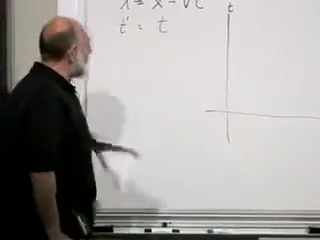
\includegraphics[width=0.72\textwidth]{lecture_04_figure_02.png}
\caption{伽利略變換與初始的$t$-$x$網格。運動的原點會沿著$x=vt$前進，而兩個參考系仍共用相同的等時線。}
\lectureframe{00:03:06}
\end{figure}

由式~\eqref{eq:l4-galilean}解出不帶撇號的座標，得到
\begin{align}
x&=x'+vt'=x'+vt, & t&=t'.
\end{align}
逆變換的形式相同，只要將$v$換成$-v$即可。如果列車相對車站向前運動，那麼車站相對列車便向後運動。在狹義相對論中，這種互易性依然成立，但普適時間則不成立。

\section{洛倫茲修正}

伽利略變換無法使光速在每個慣性參考系中都相同。修正後的關係式先寫成$c=1$單位制下的形式：
\begin{align}
x'&=\frac{x-vt}{\sqrt{1-v^2}}, &
t'&=\frac{t-vx}{\sqrt{1-v^2}}.
\label{eq:l4-lorentz-natural}
\end{align}
恢復一般單位制後，得到
\begin{align}
x'&=\frac{x-vt}{\sqrt{1-v^2/c^2}}, &
t'&=\frac{t-vx/c^2}{\sqrt{1-v^2/c^2}}.
\label{eq:l4-lorentz-c}
\end{align}

\begin{figure}[H]
\centering
\includegraphics[width=0.74\textwidth]{lecture_04_figure_05.png}
\caption{補回$c$因子的洛倫茲變換。}
\lectureframe{00:09:10}
\end{figure}

當$v\ll c$時，在適用牛頓力學的情況下，$v^2/c^2$和$vx/c^2$都很小。此時，式~\eqref{eq:l4-lorentz-c}便還原為伽利略變換的結果。相對論並未摒棄牛頓運動學，而是指出了它的適用範圍。

當$v=c$時，分母為零。慣性參考系不可能相對另一個慣性參考系以光速運動。遠低於此極限時，修正很小；但接近極限時，$x$與$t$的混合便無可避免。

運動方向選在$x$，因此橫向座標不變：
\begin{equation}
y'=y,\qquad z'=z.
\end{equation}
可以用以下方式理解原因：在列車和月台上各放一根相同的橫向米尺。一位以兩個參考系速度中間值運動的觀測者，會看到兩根尺以大小相等、方向相反的速度彼此接近。這個安排沒有任何特徵會使其中一根橫向米尺比另一根短。

\section{沿光錐方向的洛倫茲變換}

式~\eqref{eq:l4-lorentz-natural}還有一種幾何上的讀法。將其中兩個方程相加：
\begin{align}
t'+x'
&=\frac{(t-vx)+(x-vt)}{\sqrt{1-v^2}}\\
&=(t+x)\frac{1-v}{\sqrt{1-v^2}}\\
&=(t+x)\sqrt{\frac{1-v}{1+v}}.
\label{eq:l4-null-plus}
\end{align}
再以相反的順序相減：
\begin{align}
t'-x'
&=\frac{(t-vx)-(x-vt)}{\sqrt{1-v^2}}\\
&=(t-x)\frac{1+v}{\sqrt{1-v^2}}\\
&=(t-x)\sqrt{\frac{1+v}{1-v}}.
\label{eq:l4-null-minus}
\end{align}

\begin{figure}[H]
\centering
\includegraphics[width=0.75\textwidth]{lecture_04_figure_06.png}
\caption{以零座標組合$t+x$和$t-x$重寫的洛倫茲變換。兩者的比例因子互為倒數。}
\lectureframe{00:18:45}
\end{figure}

組合$t+x$和$t-x$是沿著兩個$45^\circ$類光方向的座標。洛倫茲推進會壓縮其中一個方向，並以互為倒數的因子拉伸另一個方向。兩個方向都不會偏離$45^\circ$。因此光線仍是光線；這正是光速不變性在時空中的圖像。

\begin{classroomqa}
\audiencequestion{位於中間的觀測者看到一個對稱的實驗，但這如何證明列車與月台上的觀測者也會得到相同結果？\lecturetimestamp{00:20:48}}
\lecturerresponse{這裡還用到另一項事實：事件是否重合是不變的。如果兩根尺的端點相遇，那次相遇就是一個時空事件。每位慣性觀測者都可以為它指定不同的座標，但沒有人能把一次重合拆成發生在兩個不同位置的事件。在相應端點相遇處發出的閃光，能讓這些事件在實際上被探測到。中間參考系的對稱性，加上兩個端點相遇事件的不變性，便確立了兩根尺的橫向長度相同。}
\end{classroomqa}

\begin{classroomqa}
\audiencequestion{代表中間參考系的騎腳踏車者，必須實際位於兩根尺的中點嗎？\lecturetimestamp{00:22:25}}
\lecturerresponse{不必。參考系是一整個由觀測者和時鐘構成的網絡，不是某個位置上的一隻眼睛。騎腳踏車者可以稍後才收到端點發出的閃光，再推斷閃光的發射位置。關鍵是每個發射事件在時空中的位置，而不是光最後在哪裡被接收。}
\end{classroomqa}

連續速度的合成也是同一變換的推論之一，但這部分刻意留到下一講再談。現在要做的是找出運動時鐘所測量的不變量。

\section{不變間隔}

普通笛卡兒座標軸旋轉時，量$x^2+y^2$保持不變。洛倫茲變換保留的則是另一種二次型。由式~\eqref{eq:l4-lorentz-natural}可得：
\begin{align}
t'^2-x'^2
&=\frac{(t-vx)^2-(x-vt)^2}{1-v^2}\\
&=\frac{t^2-2vtx+v^2x^2-x^2+2vtx-v^2t^2}{1-v^2}\\
&=t^2-x^2.
\label{eq:l4-interval}
\end{align}
混合項彼此抵消，剩下的分子則含有公因子$1-v^2$。

\begin{figure}[H]
\centering
\includegraphics[width=0.76\textwidth]{lecture_04_figure_07.png}
\caption{黑板上推導$t'^2-x'^2=t^2-x^2$的過程。}
\lectureframe{00:33:15}
\end{figure}

在三維空間中，不變量為
\begin{equation}
t'^2-x'^2-y'^2-z'^2=t^2-x^2-y^2-z^2
\end{equation}
此處採用$c=1$單位制。更一般地，對兩個事件，我們使用座標差：
\begin{equation}
\Delta s^2
=c^2\Delta t^2-\Delta x^2-\Delta y^2-\Delta z^2.
\label{eq:l4-spacetime-interval}
\end{equation}
每位慣性觀測者對這個數值都一致，儘管他們對時間項和空間項各自的數值並不一致。

\section{固有時與運動時鐘}

想像一個由靜止觀測者組成的格點，他們已透過交換光訊號將時鐘同步。他們的時鐘讀數定義了座標時間$t$。現在讓一只手錶穿過這個格點。手錶沿著自己的世界線前進，其自身的讀數就是固有時。

對兩個類時分離的事件，定義
\begin{equation}
c^2\Delta\tau^2
=c^2\Delta t^2-\Delta x^2-\Delta y^2-\Delta z^2.
\label{eq:l4-proper-time}
\end{equation}
在一維空間且採用$c=1$單位制時，這個定義簡化為
\begin{equation}
\Delta\tau=\sqrt{\Delta t^2-\Delta x^2}.
\end{equation}
它的平方根形式類似普通距離的公式，但負號改變了幾何性質。

有三種情況：
\begin{align}
\Delta t^2-\Delta x^2 &>0 &&\text{timelike},\\
\Delta t^2-\Delta x^2 &=0 &&\text{lightlike},\\
\Delta t^2-\Delta x^2 &<0 &&\text{spacelike}.
\end{align}
在光錐內部，固有時為實數。在光錐上，也就是$x=\pm t$的位置，即使兩個事件不必重合，固有時仍為零。光線恰好可以連接這樣的事件。在光錐外部，間隔是類空的；用實數固有距離$\sqrt{\Delta x^2-\Delta t^2}$描述會比用虛數的時鐘時間恰當。

\begin{figure}[H]
\centering
\includegraphics[width=0.73\textwidth]{lecture_04_figure_08.png}

\vspace{0.8em}

\begin{tikzpicture}[x=1.0cm,y=1.0cm]
\draw[->] (-3.3,0) -- (3.3,0) node[right] {$x$};
\draw[->] (0,-0.4) -- (0,4.0) node[above] {$t$};
\draw[thick] (0,0) -- (3.0,3.0) node[above right] {$x=t$};
\draw[thick] (0,0) -- (-3.0,3.0) node[above left] {$x=-t$};
\node at (0,2.0) {timelike};
\node at (2.25,1.05) {spacelike};
\node at (-2.25,1.05) {spacelike};
\end{tikzpicture}
\caption{黑板上的光錐，以及對類時、類光與類空間隔的清楚分類。}
\lectureframe{00:38:40}
\end{figure}

為什麼式~\eqref{eq:l4-proper-time}等於時鐘讀數？對靜止的時鐘而言，$\Delta x=0$，所以$\Delta\tau=\Delta t$。對等速運動的時鐘，選擇一個該時鐘靜止的帶撇號參考系。在那個參考系中，$\Delta x'=0$，而不變性給出
\begin{equation}
\Delta\tau
=\sqrt{\Delta t'^2-\Delta x'^2}
=\Delta t'.
\end{equation}
因此，運動時鐘所記錄的就是固有時。

\begin{classroomqa}
\audiencequestion{``事件之間的間隔''和``時鐘的讀數''是同一事物的兩種說法嗎？
\lecturetimestamp{00:44:49}}
\lecturerresponse{理想時鐘若沿慣性運動從一個事件行至另一個事件，兩者便相等。不變間隔是幾何量；共動時鐘兩端讀數的差則是對它的物理測量。靜止的座標時鐘通常會記錄不同的座標時間間隔。}
\end{classroomqa}

\section{時間膨脹與同時性}

考慮運動參考系的原點。它的世界線滿足
\begin{equation}
x'=0,\qquad x=vt.
\end{equation}
同一條傾斜直線既是運動時鐘的路徑，也是$t'$軸。

\begin{figure}[H]
\centering
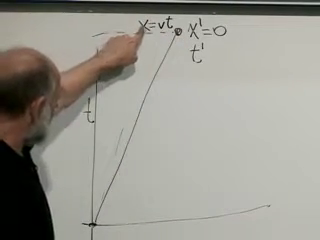
\includegraphics[width=0.72\textwidth]{lecture_04_figure_03.png}
\caption{運動原點：$x=vt$、$x'=0$和$t'$軸，都是描述同一條世界線的方式。}
\lectureframe{00:48:18}
\end{figure}

將不變間隔用於共同原點與該世界線上稍後的一點：
\begin{align}
t'^2-x'^2&=t^2-x^2,\\
t'^2&=t^2-v^2t^2,\\
t'&=t\sqrt{1-v^2}.
\label{eq:l4-time-dilation-natural}
\end{align}
補回$c$後，得到
\begin{equation}
\Delta\tau=\Delta t\sqrt{1-\frac{v^2}{c^2}}
=\frac{\Delta t}{\gamma},
\qquad
\gamma=\frac{1}{\sqrt{1-v^2/c^2}}.
\label{eq:l4-time-dilation}
\end{equation}

\begin{figure}[H]
\centering
\includegraphics[width=0.73\textwidth]{lecture_04_figure_09.png}
\caption{黑板上的時間膨脹結果：採用$c=1$單位制時，運動時鐘累積的固有時為$t'=t\sqrt{1-v^2}$。}
\lectureframe{00:50:45}
\end{figure}

靜止觀測者認為運動時鐘走得較慢。互易性要求運動觀測者也認為靜止時鐘走得較慢。這並不矛盾，因為兩種描述比較的是不同的遠距事件。

事實上，式~\eqref{eq:l4-lorentz-natural}中，$t'$為常數時滿足
\begin{equation}
t-vx=\text{constant}.
\label{eq:l4-simultaneity}
\end{equation}
運動觀測者的同時線相對於水平線$t=\text{constant}$是傾斜的。每位觀測者都把遠方時鐘讀數的不同組合視為同時。只要看清這項差異，時鐘彼此變慢的說法便不矛盾。

\begin{figure}[H]
\centering
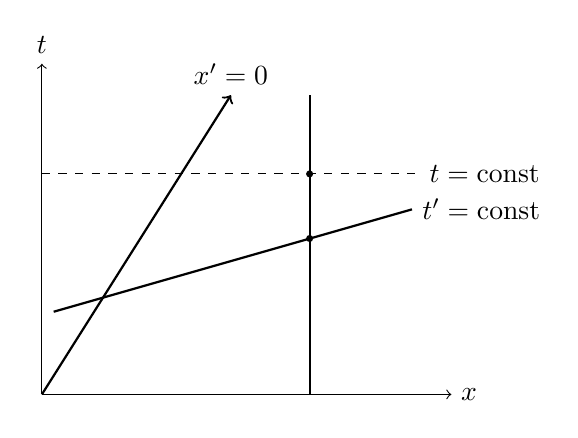
\begin{tikzpicture}[x=1cm,y=1cm]
\draw[->] (0,0) -- (0,4.2) node[above] {$t$};
\draw[->] (0,0) -- (5.2,0) node[right] {$x$};
\draw[thick,->] (0,0) -- (2.4,3.8) node[above] {$x'=0$};
\draw[dashed] (0,2.8) -- (4.8,2.8)
  node[right] {$t=\mathrm{const}$};
\draw[thick] (0.15,1.05) -- (4.7,2.35)
  node[right] {$t'=\mathrm{const}$};
\draw[thick] (3.4,0) -- (3.4,3.8);
\fill (3.4,2.8) circle (0.045);
\fill (3.4,1.98) circle (0.045);
\end{tikzpicture}
\caption{互易的時間膨脹，是在不同的同時性切片上比較時鐘讀數。}
\end{figure}

\section{雙胞胎的路徑}

兩位雙胞胎從同一事件出發。一位留在$x=0$。另一位以速度$v$向外行進，接著掉頭，再以相同速度返回。重逢時，他們比較所有可作為時鐘的物理過程：手錶、心跳、新陳代謝，或衰老本身。

令旅程的每一段在留守者的參考系中都歷時$T$座標時間。留守雙胞胎的固有時為
\begin{equation}
\tau_{\mathrm{home}}=2T.
\end{equation}
掉頭事件的座標為$(vT,T)$。因此，外出路程所累積的固有時為
\begin{align}
\tau_{\mathrm{leg}}
&=\sqrt{T^2-v^2T^2}
=T\sqrt{1-v^2}.
\end{align}
回程也累積相同的固有時，所以
\begin{equation}
\tau_{\mathrm{travel}}=2T\sqrt{1-v^2}<2T.
\label{eq:l4-twin}
\end{equation}

\begin{figure}[H]
\centering
\includegraphics[width=0.73\textwidth]{lecture_04_figure_10.png}

\vspace{0.8em}

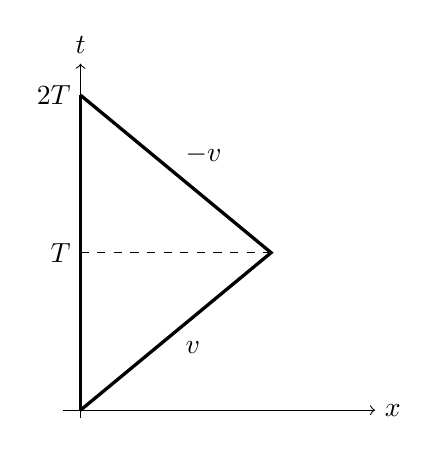
\begin{tikzpicture}[x=1.1cm,y=1cm]
\draw[->] (-0.2,0) -- (3.4,0) node[right] {$x$};
\draw[->] (0,-0.1) -- (0,4.4) node[above] {$t$};
\draw[very thick] (0,0) -- (0,4);
\draw[very thick] (0,0) -- (2.2,2) -- (0,4);
\draw[dashed] (0,2) -- (2.2,2);
\node[left] at (0,2) {$T$};
\node[left] at (0,4) {$2T$};
\node[below right] at (1.1,1.0) {$v$};
\node[above right] at (1.1,3.0) {$-v$};
\end{tikzpicture}
\caption{留守者的世界線與雙胞胎外出的兩段路程。它們的固有時不同，因為它們是穿越時空的不同路徑。}
\lectureframe{00:59:35}
\end{figure}

雙胞胎年齡不同並不矛盾。旅行路徑包含一次轉向，因此無法透過單一慣性參考系對稱性，將它與留守者的直線路徑聯繫起來。在普通歐幾里得幾何中，連接兩點的直線路徑與折線路徑長度也不同。閔可夫斯基幾何中，哪條路徑的間隔較大恰好相反，但比較仍是幾何上的比較。

\section{加速度與理想時鐘}

\begin{classroomqa}
\audiencequestion{在掉頭時，物理情況有所不同，旅行者也會加速。這會使時鐘計算失效嗎？
\lecturetimestamp{01:02:19}}
\lecturerresponse{加速度是真實的，也有助於辨認不對稱性；不應把它搪塞過去。尖銳的轉角只是理想化的圖示，可以改成有限時間內平順完成的轉向。還需要一項物理假設：尺寸足夠小、構造良好的時鐘不受適度加速度影響，並會繼續記錄固有時。大型或脆弱的時鐘可能變形或損壞，但那是時鐘機制的缺陷，而非時空間隔的問題。}
\end{classroomqa}

理想時鐘這項假設無法單從洛倫茲變換推導出來，而是透過實際時鐘機制的行為加以檢驗。原子比一個橫跨數百英里的時鐘更接近理想時鐘，因為緊密的機制較不容易在加速度或重力作用下變形。只提到廣義相對論，並不能消除這個物理問題；我們仍須了解所選機制如何對環境作出反應。

\begin{classroomqa}
\audiencequestion{能否把加速軌跡分成許多短區段，使每一段仍可使用慣性分析？\lecturetimestamp{01:09:08}}
\lecturerresponse{可以。將曲線分成短而近似筆直的區段，計算每一段的固有時，再把結果相加。這相當於在時空中用許多短線段求出普通曲線的長度。取連續極限時，
\[
\tau=\int \sqrt{1-\frac{v(t)^2}{c^2}}\,dt,
\]
適用於以慣性座標系描述的平直時空中的運動。}
\end{classroomqa}

\section{雙胞胎看到的情形}

可以透過發送光脈衝，實際比較最後的時鐘讀數。在兩條世界線上每隔一秒固有時做一個記號，並讓每位雙胞胎在每個記號處發出脈衝。外出途中，收到對方脈衝的間隔會拉長；回程時，脈衝則會密集到達。這就是直接呈現在時空圖上的相對論多普勒效應。

\begin{figure}[H]
\centering
\includegraphics[width=0.73\textwidth]{lecture_04_figure_11.png}
\caption{留守者與旅行者的世界線之間交換的光訊號。外出途中稀疏到達的脈衝，以及回程途中密集到達的脈衝，涵蓋了每一個發出的脈衝。}
\lectureframe{01:12:55}
\end{figure}

故事中的任何參考系都沒有消失。每位觀測者最終都會收到對方發出的所有脈衝，但接收速率取決於相對運動。對兩條路徑而言，外出時的紅移與回程時的藍移持續時間不同，因此把收到的脈衝全部計數後，仍會符合固有時的比較結果。

\begin{classroomqa}
\audiencequestion{回程的旅行者若收到藍移的光，會不會收集到比光源發出時更多的能量？\lecturetimestamp{01:13:50}}
\lecturerresponse{要回答這個問題，必須先建立能量的相對論定義及其參考系依賴性；目前尚未討論這些內容。這個問題問得合理，但單靠座標和脈衝計數不足以釐清能量帳目，尤其對加速中的觀測者更是如此。因此應該暫緩回答，而不是猜測。}
\end{classroomqa}

\section{閉合的空間方向}

\begin{classroomqa}
\audiencequestion{假設有一個緊緻化的空間方向。雙胞胎能否沿這個方向等速運動、回到出發地，完全不經歷加速度？那麼，兩位雙胞胎有何不同？\lecturetimestamp{01:15:14}}
\lecturerresponse{應將空間本身想像成一個圓柱面，而不是彎曲後嵌入更大空間中的一張面；這裡不需要徑向加速度。然而，返回的觀測者仍會遇到同一地點反覆出現這項全域特性。這顯示存在某種不對稱性，但若要完整回答，就必須仔細處理具有空間識別的狹義相對論。這裡先把問題保留為開放問題，不臨時拼湊答案。}
\end{classroomqa}

\begin{figure}[H]
\centering
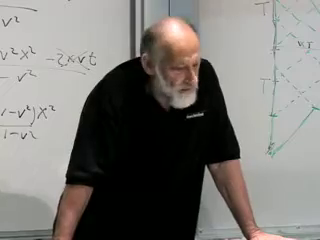
\includegraphics[width=0.72\textwidth]{lecture_04_figure_04.png}

\vspace{0.8em}

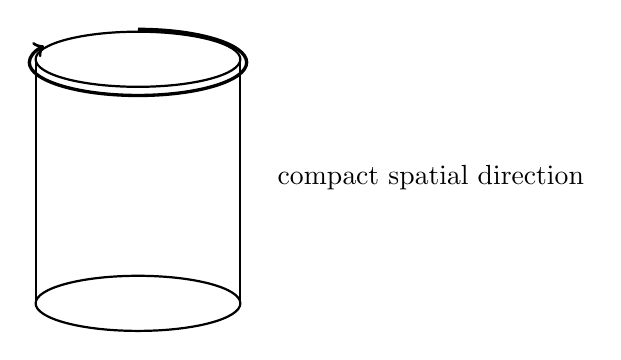
\begin{tikzpicture}[x=1cm,y=1cm]
\draw[thick] (0,0) ellipse (1.3 and 0.35);
\draw[thick] (-1.3,0) -- (-1.3,-3.1);
\draw[thick] (1.3,0) -- (1.3,-3.1);
\draw[thick] (0,-3.1) ellipse (1.3 and 0.35);
\draw[->,very thick] (0.0,0.38) arc (90:-210:1.38 and 0.42);
\node[right] at (1.65,-1.5) {compact spatial direction};
\end{tikzpicture}
\caption{黑板上畫出的緊緻空間問題，並以清楚的內在圓柱面呈現。這是關於全域識別的問題，而非關於在額外的徑向維度中繞著圓柱面運動。}
\lectureframe{01:17:56}
\end{figure}

\section{長度是在同時性切片上測量的}

處理狹義相對論問題時，先畫出時空圖。取一根在不帶撇號參考系中靜止的米尺，兩端位於$x=0$和$x=1$。隨著時間經過，兩個端點各自描出垂直的世界線。米尺在兩條世界線之間掃出一條帶狀區域。

運動觀測者必須在運動時間$t'$的同一時刻測量兩個端點。由式~\eqref{eq:l4-simultaneity}可知，通過原點且滿足$t'=0$的切片，在$c=1$單位制下符合
\begin{equation}
t=vx
\end{equation}
這個切片與右端點$x=1$的世界線相交於$t=v$。

\begin{figure}[H]
\centering
\includegraphics[width=0.73\textwidth]{lecture_04_figure_12.png}

\vspace{0.8em}

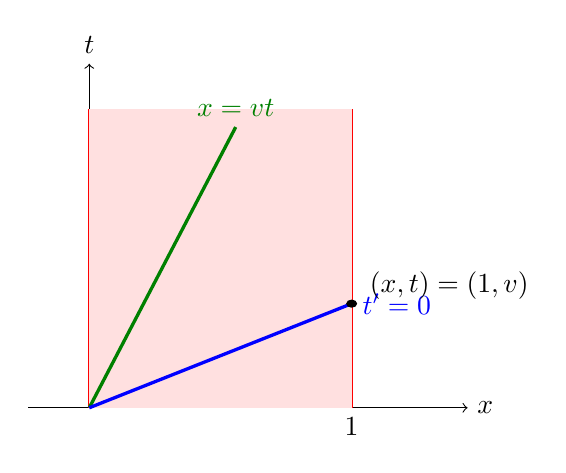
\begin{tikzpicture}[x=1.55cm,y=1.15cm]
\draw[->] (-0.5,0) -- (3.1,0) node[right] {$x$};
\draw[->] (0,0) -- (0,3.8) node[above] {$t$};
\draw[very thick,red] (0,0) -- (0,3.3);
\draw[very thick,red] (2.15,0) -- (2.15,3.3);
\fill[red!12] (0,0) rectangle (2.15,3.3);
\draw[very thick,green!50!black] (0,0) -- (1.2,3.1)
  node[above] {$x=vt$};
\draw[very thick,blue] (0,0) -- (2.15,1.15)
  node[right] {$t'=0$};
\fill (2.15,1.15) circle (0.045);
\node[right] at (2.22,1.35) {$(x,t)=(1,v)$};
\node[below] at (2.15,0) {$1$};
\end{tikzpicture}
\caption{靜止的尺在時空中掃出一條帶狀區域。運動觀測者測得的長度，是尺的兩端在同一個$t'=\mathrm{const}$切片上的間距。}
\lectureframe{01:24:20}
\end{figure}

選取的端點間隔是類空的，因此使用不變量的正空間形式：
\begin{equation}
x'^2-t'^2=x^2-t^2.
\end{equation}
在選取的端點處，$t'=0$、$x=1$，且$t=v$。因此
\begin{align}
x'^2&=1-v^2,\\
x'&=\sqrt{1-v^2}.
\end{align}
於是，靜止長度為$L$的尺，在運動參考系中測得的長度為
\begin{equation}
L'=L\sqrt{1-v^2/c^2}=\frac{L}{\gamma}.
\label{eq:l4-length-contraction}
\end{equation}

\begin{figure}[H]
\centering
\includegraphics[width=0.76\textwidth]{lecture_04_figure_13.png}
\caption{完成的長度收縮作圖，以及靜止長度為一單位時黑板上得到的結果$x'=\sqrt{1-v^2}$。}
\lectureframe{01:28:10}
\end{figure}

互易的說法也成立：月台上的觀測者測得列車上的縱向米尺較短。再一次，兩位觀測者選取了不同的同時端點事件，因此互易性並不矛盾。

\section{最後的問題}

\begin{classroomqa}
\audiencequestion{除了光，還有什麼會以光速傳播？特別是引力呢？\lecturetimestamp{01:29:29}}
\lecturerresponse{廣義相對論預言，引力波會以$c$傳播。在這場講座舉行時，相關證據來自雙脈衝星等系統的間接觀測；當時尚未直接探測到引力波。\editorialnote{這場2006講座之後，實驗情況有所改變。LIGO 在 2015 年直接探測到 GW150914；而在 2017 年對 GW170817 及其電磁對應訊號的聯合觀測，顯示引力與光的傳播速度差異僅在 $10^{15}$ 分之幾的量級。參見 \url{https://ligo.org/detections/gw150914/} 和
\url{https://doi.org/10.1103/PhysRevLett.119.251302}。}}
\end{classroomqa}

\begin{classroomqa}
\audiencequestion{太空人能否在少於以光年表示的距離數值所對應的固有時內，穿越數光年的距離？這是否代表他移動得比光還快？\lecturetimestamp{01:30:38}}
\lecturerresponse{太空人的固有時為
$\sqrt{\Delta t^2-\Delta x^2}$，小於座標時間$\Delta t$。在太空人的慣性參考系中，恆星之間的距離會發生洛倫茲收縮。恆星以速度$-v$運動，並未超過光速；只是需要穿越的收縮後距離較短。}
\end{classroomqa}

如果太空人從靜止開始加速，描述就會隨著一系列瞬時慣性參考系而改變。在這段轉換過程中，恆星之間的距離可能改變。不能用單一固定的洛倫茲變換描述整段加速歷程，但總固有時仍可由沿世界線累加各段貢獻求得。真實的雙胞胎也是如此：他會起航、轉向並減速，而不是一出生就以巡航速度行進。

\begin{classroomqa}
\audiencequestion{這些難題是否源於把時間視為特殊的存在？我們是否必須稱它為第四維？\lecturetimestamp{01:36:43}}
\lecturerresponse{不必一開始就採用「時間是第四維」這句口號。洛倫茲變換本身就迫使空間與時間混合，而間隔$t^2-x^2-y^2-z^2$則把兩者視為同一幾何的組成部分，只是時間項與空間項的符號不同。在低速下，這種混合可以忽略，熟悉的牛頓直覺便會恢復。但在相對論速度下，空間與時間不能被視為根本上彼此獨立。}
\end{classroomqa}

因此，時間膨脹、長度收縮、雙胞胎的比較，以及縮短的旅行時間，並非彼此無關的技巧。它們都源自三個做法：辨明要比較的事件、畫出事件的時空幾何，並使用不變間隔。